\chapter{资源受限终端任务调度策略}\label{chap:task_scheduling}

\section{引言}

任务调度问题是指系统在同时接收到多个服务请求任务的时候,将这些任务合理地分配给多个智能终端上的容器进行处理,由于不同的容器所在智能终端的处理能力不同,每个容器所占用的资源也不同,导致不同的调度方案结果会有差异,需要针对在容器化智能终端协同服务场景下的一些特点来进行取舍和进一步的优化,以追求对于终端资源利用的最大化。在该任务场景下,最常见的用户需求就是实时性需求,也即要求任务能够被快速响应、快速执行、且执行结果能够快速回传给用户,因此最小化任务完成时间是任务调度问题最主要的目标。除此之外,需要考虑的因素还涉及硬件设备功耗、分布式设备负载均衡度等。

\section{相关工作}

\subsection{传统任务调度问题求解方法}

任务调度问题是NP-hard问题,已有的任务调度算法主要分为两大类,一类是基于局部贪心策略的算法,另一类是启发式的智能搜索方法。贪心策略的算法,例如优先调度任务量最重的算法,或者优先调度计算时间最短的算法,其调度结果很容易陷入局部最优解,不能够合理利用所有资源。启发式算法则是确定搜索策略,通过迭代、评价等方式,逐步逼近全局最优解。

任务调度问题是将多个任务计划到约束下的多个节点的问题。任务调度问题是一个优化问题。应用多种算法来解决任务调度问题。基于最佳资源选择 (BRS) 的算法, 如最大最小、最小、苦难等, 是解决任务调度问题的传统方法。一些元启发式算法, 如 PSO 和基于 pso 的改进算法, 是处理任务调度问题的新方法。

\subsection{启发式算法求解方法}

近年来, 对任务调度问题进行了大量的研究。随着研究的进行, 许多元启发式算法被用来处理复杂的优化问题。元启发式算法具有简单的操作和较少的开销, 能够找到全局最优。

启发式算法中,如遗传算法(Genetic Algorithm),是模拟达尔文生物进化论的自然选择和遗传学机理的生物进化过程的计算模型,通过模拟自然进化过程搜索最优解。遗传算法将一个调度方案表示为一个染色体,并利用交叉、变异等运算符实现调度方案的进化,最终得到的结果比较好,但是收敛速度较慢且运算量较大。模拟退火算法(Simulated Annealing Algorithm),仿照固体退火原理,是一种基于概率的算法,从某一较高初温出发,伴随温度参数的不断下降,结合概率突跳特性在解空间中随机寻找目标函数的全局最优解,即在局部最优解能概率性地跳出并最终趋于全局最优。Kennedy和Eberhart在1995年提出粒子群算法(Particle Swarm Optimization),该算法最初是受到飞鸟集群活动的规律性启发,进而利用群体智能建立的一个简化模型,通过追随当前搜索到的最优值来寻找全局最优。

许多元启发式算法被引入到优化问题中。GA 是戈德伯格在1988年提出的经典元启发式算法, 它将自然选择理论引入到优化过程中, 包括突变、交叉和选择 \ citefonseca1995an,Whitley1994, Tanese1989DGA, Ng广州市2018。虽然 GA 的性能相当好, 但遗传算法的操作过于复杂, 无法实现, 不适合某些情况。一些元启发式算法的灵感来自昆虫、鱼类、鸟类和其他群体生物的自然行为。粒子群算法 (PSO) 是肯尼迪1995年提出的经典元启发式算法。PSO 的原理简单, 性能显著 \ 1995年的柠檬素颗粒, Liao2007, Gomathi2013。蚁群优化算法 (ACO) 是受蚂蚁在鸟巢和食物来源之间自然觅食行为的启发。ACO 利用化学信息素在中国的人群中进行交流。

最近提出了一些新的元启发式优化算法。关于改进这些算法的研究并不多。蚂蚁狮子优化器提出 (ALO) 在2015年是受狮子 \ citemirjilili2013 蚂蚁的狩猎行为的启发。鲸鱼优化算法 (WOA) 于2016年提出。WA 模拟鲸鱼的自然狩猎行为。2016年提出的蜻蜓算法 (DA) 是受蜻蜓群在自然界中的静态和动态行为的启发。


2017年, Shahrzad Saremi 和 Seyedali Mirjalili 提出了一种新的元启发式优化算法, 称为蝗虫优化算法 (GOA)。GOA 利用群体内部的相互作用和蜂群外的风的影响来模拟蝗虫群的迁徙行为, 寻找目标食物 \ citesare2013 2017 蝗虫。GOA 算法利用群智能, 通过在蝗虫群之间分享经验, 确定搜索方向, 找到最佳或近似的最佳位置。GOA 还使用了具有多个迭代的进化方法, 以提高群智能的效率。

开发了一些基于 GOA 的改进算法。OBLGOA 是由艾哈迈德·埃维斯在2018年提出的 \ ceewees 2013 改进。根据目前的搜索位置, 引入了基于对立面的学习策略, 以生成相反的解作为候选方案。OBL 策略可以提高算法的收敛速度, 但由于缺乏随机性, 改进有限。桑卡拉阿罗拉提出了混沌蝗虫优化算法在 2018年 \ 柠檬酸乱糟糟。将混沌映射应用到算法中, 提高了 GOA 的性能。采用10幅混沌映射来评价混沌理论的影响。结果并不是特别理想, 因为混沌因素在处理许多基准函数时并不合适。提出了一种基于 GOA 的新算法来解决优化问题和任务调度问题。

\section{GOA算法}

蝗虫优化算法模拟蝗虫的昆虫群行为。蝗虫蜂拥而至, 远距离迁徙, 寻找一个有食物的新栖息地。在这个过程中, 蝗虫之间的互动在蜂群内部互相影响。风的力量和蜂群外的重力影响蝗虫的轨迹。食物的目标也是一个重要的影响因素。

受上述三个因素的影响, 移民过程分为勘探和开发两个阶段。在勘探阶段, 鼓励蝗虫快速、突然地移动, 寻找更多潜在的目标区域。在开发阶段, 蝗虫往往在当地移动, 以寻找更好的目标地区。蝗虫自然实现了勘探开发寻找食物来源的两种迁徙趋势。此过程可以抽象为优化问题。蝗虫群被抽象为一群搜索代理。

Seyedali Mirjalili 在文献[]中提出了蝗虫群体迁移的数学模型。具体的模拟公式如下:

\begin{equation}
    X_i = S_i + G_i + A_i 
\end{equation}

这里变量$X_i$是第i个搜索单位的位置,变量$S_i$代表蝗虫集群内部搜索单位间社会交互对第i个搜索单位的影响因子,变量$G_i$代表蝗虫集群外部重力因素对第i个搜索单位的影响因子,变量$A_i$代表风力的影响因子。变量$S_i$的定义公式如下:

\begin{equation}
    S_i = \sum_{j=1, j\neq{i}}^N s(d_{ij})\widehat{d_{ij}}
\end{equation}

这里变量$d_{ij}$代表第i个搜索单位和第j个搜索单位之间的欧式距离,计算方法如下:
\begin{equation}
    d_{ij}=|x_j-x_i|
\end{equation}

变量$\widehat{d_{ij}}$代表第i个搜索单位和第j个搜索单位之间的单位向量,计算方法如下:

\begin{equation}
    \widehat{d_{ij}}=\frac{x_j-x_i}{d_{ij}}
\end{equation}

\emph{s}是一个函数,用于计算蝗虫集群之间的社会关系影响因子,该函数定义如下:

\begin{equation}
    s(r) = fe^{\frac{-r}{l}}-e^{-r}
\end{equation}

这里\emph{e}是自然底数,变量\emph{f}代表吸引力因子,参数\emph{l}代表吸引力长度。
% where \emph{e} is the Natural Logarithm, \emph{f} represents the concentration of attraction and the parameter of \emph{l} shows the attractive length scale.
当应用于解决数学优化问题的时候,为了优化数学模型,公式1中需要加入一些适当的改动。代表集群外部影响因子的变量$G_i$和$A_i$需要被替换为目标食物的位置。这样计算公式就变成了如下的样子:

\begin{equation}
    x_i = c \Bigl(\sum_{j=1,j\neq{i}}^N c \frac{u-l}{2}s (\lvert x_j-x_i \rvert )\frac{x_j-x_i}{d_{ij}} \Bigr) + \widehat{T_d}
\end{equation}

这里参数\emph{u}和参数\emph{l}分别代表搜索空间的上界和下界。变量$\widehat{T_d}$是目标食物的位置,在优化问题的数学模型中代表所有搜索单位在整个搜索过程中所能找到的最优的解的位置。另外,参数\emph{c}是搜索单元的搜索舒适区控制参数,改变参数\emph{c}的大小可以平衡搜索过程中的“开拓”和“探索”两个阶段。参数\emph{c}的计算方式如下:

\begin{equation}
    c = cmax - iter \frac{cmax - cmin}{MaxIteration}
\end{equation}


这里参数\emph{cmax}和参数\emph{cmin}分别是参数\emph{c}的最大值和最小值,参数\emph{iter}代表当前的迭代次数,参数\emph{MaxIteration}代表最大迭代次数。

在优化问题的求解过程中,公式4作为演进公式,被不断循环迭代来寻找最优解,直到达到迭代终止条件为止。通常迭代终止条件为达到预设的最大迭代次数,或者所得到的最优解满足预设的最优解条件。在本研究所涉及到的优化问题中,迭代终止条件均为达到预设的最大迭代次数。在迭代演进的过程结束后,该算法可以得到一个近似的最优解的位置以及相应的最优解的值。

蝗虫优化算法的算法伪代码如算法1所示:
\begin{algorithm}
    % \setstretch{1.35}

    \caption{蝗虫优化算法}
    \label{alg:GOA}
    
    \begin{algorithmic}[1]
    \State initialize the swarm and set the position boundaries u and l
    \State initialize the factors including cmax, cmin, MaxIteration
    \State initialize all the search agents position with random origin matrix 
    \State calculate the target fitness and mark the target position
    
    \While {$(iter < MaxIteration$ and $target fitness > destination fitness)$}
    \State calculate $d_ij$ and $\widehat{d_ij}$ by equation(2)
    \State calculate $s(d_ij)$ by equation(3)
    \State update $x_i$ by equation(4)
    \State calculate the fitness 
    \If{current fitness is better than target fitness}
        \State update the target fitness and the target position
    \EndIf
    \State $iter = iter +1$
     
    \EndWhile

    \State Return target fitness and target position
    
    
    \end{algorithmic}
    
\end{algorithm}

\subsection{蝗虫算法优缺点分析}
GOA是最近受到蚱蜢自然迁移行为启发的元启发式算法。 虽然GOA具有简单的理论基础并且易于实现,但GOA的性能更优越。 原始的GOA改变了蚱蜢的舒适区域,这可以使目标通过迭代收敛到全局最优解。 与一些经典算法相比,GOA的收敛速度要快得多。 GOA可显着提高蝗虫的平均适应度,改善蝗虫的初始随机种群。虽然GOA具有这些优点,但它也存在一些阻碍算法获得更好解决方案的缺点。 在对GOA公式进行一些理论分析和用MATLAB代码进行的一些实验之后,给出了GOA的几个缺点。

首先,GOA使用线性递减参数使搜索过程收敛,这很难区分过程的两个阶段,即开发阶段和探索阶段。 其次,在搜索过程的早期阶段的每次迭代期间,最佳解决方案的位置急剧波动。 似乎最终的最佳解决方案只受搜索过程后期的影响,无论前一阶段的结果如何。 GOA理论无法充分利用所有搜索迭代。 当最大迭代次数增加时,GOA的最佳适应性不是很突出,例如,从实验结果中发现的500到1500。 最后,搜索过程很容易陷入局部最优。 GOA易于实现的优势无助于摆脱局部最优,这可能是GOA的劣势。


\section{带随机跳出机制的动态权重蝗虫优化算法}
\subsection{动态权重}
GOA使用线性递减参数来限制搜索空间并使所有搜索代理移动到目标位置。 线性递减参数不能增强搜索过程的两个阶段的影响,即开发阶段和探索阶段。 在探索阶段,GOA无法在目标搜索区域周围快速收敛,搜索代理只是在整个搜索空间中游荡,这无法为后期搜索阶段奠定坚实的基础。 在开发阶段,参数通常使搜索代理滑过局部最佳位置,就像搜索代理超速运动一样。

线性递减参数机制无法使算法充分利用整个迭代。 引入动态权重参数机制以提高算法的利用率。 搜索进度分为三个阶段,即早期阶段,中间阶段阶段和后期阶段。 在早期阶段,目标位置的权重应该更高,以使搜索过程快速收敛。 在中间阶段,参数应该是稳定的,以使算法探索搜索空间。 在后期阶段,搜索代理中的重力的权重应该更小,以深入利用局部最优解位置。 具有动态权重参数的GOA公式表示为算法[1]。 新的迭代方程如下:

\begin{equation}
    x_i = m*c \Bigl(\sum_{j=1,j\neq{i}}^N c \frac{u-l}{2}s (\lvert x_j-x_i \rvert )\frac{x_j-x_i}{d_{ij}} \Bigr) + \widehat{T_d}
\end{equation}
where \emph{m} is the dynamic weight parameter to adjust the search process. To correspond to the feature of the three phases of the search process, the parameter \emph{m} is set as follows:
\begin{equation}
    m= \begin{cases}
        0.5-\frac{(0.5-0.1)*iter}{MaxIteration*0.2} & \quad 0<iter\leq MaxIteration*0.2 \\
        0.1&\quad MaxIteration*0.2<iter \leq MaxIteration*0.8 \\
        0.05& \quad  MaxIteration*0.8 < iter \leq MaxIteration
        \end{cases} 
\end{equation}

\subsection{随机跳出机制}

原始的GOA算法没有使用跳跃机制,并且所有搜索代理仅根据社交互动和目标食物吸引力的影响而移动。 原始GOA的机制可能导致算法陷入局部最优位置。

引入随机跳跃策略以帮助GOA算法提高跳出局部最佳位置的概率。 参数\emph{p}被设置为跳跃阈值。 在迭代结束之前,将当前最佳适合度与最后一次迭代的最佳适应度进行比较。 如果当前最佳适应度和最后一个最佳适应度的比率高于阈值\emph{p},则可以假设该算法没有找到更好的解决方案,并且随机跳跃机制应该启动。 根据随机初始化规则在最佳位置周围生成新的搜索代理。 随机初始化规则如下:
\begin{equation}
    tempPos=curPos*((0.5-rand)*iniRan+1);
\end{equation} 
其中\emph{tempPos}是新搜索代理的位置,\emph{curPos}是当前最佳解决方案的位置。 \emph{iniRan}是管理随机跳跃边界的初始化范围参数。 如果\emph{iniRan}更高,则算法的全局搜索能力就像模拟退火算法一样得到增强。
\subsection{DJGOA算法流程}

本文提出了一种随机跳跃动态权重蝗虫优化算法(DJGOA)。 DJGOA的过程分为初始阶段,参数设置阶段,计算阶段和适应度更新阶段四个阶段。在初始化阶段,设置包括位置边界在内的一些因素,并在边界内随机初始化原始群体位置。在参数设置阶段,搜索过程进入迭代循环,动态权重参数根据当前迭代由\ emph {equation(7)}设置。在计算阶段,群体内的社会交互由\ emph {equation(6)}计算。在适应度更新阶段,如果当前适应度优于历史的最佳目标适应度,则更新目标解决方案的适合度。如果当前适应度与最后一次迭代的适应度之比高于之前设置的阈值\ emph {p},则使用随机跳转策略生成新的搜索代理以尝试跳出局部最优位置通过\ emph {equation(8)}。具有随机跳跃的动态权重蝗虫优化算法(DJGOA)的伪代码显示为算法\ref{alg:DJGOA}。

\begin{algorithm}
    % \setstretch{1.35}

    \caption{带随机跳出机制的动态权重蝗虫优化算法}
    \label{alg:DJGOA}
    
    \begin{algorithmic}[1]
    
    \State initialize the swarm and set the position boundaries u and l
    \State initialize the factors including cmax, cmin, MaxIteration and iniRan
    \State initialize all the search agents position with random origin matrix 
    \State calculate the target fitness and mark the target position
    
    \While {$(iter < MaxIteration$ and $target fitness > destination fitness)$}
    \State set the dynamic weight parameter m by equation(7)
    \State calculate $d_ij$ and $\widehat{d_ij}$ by equation(2)
    \State calculate $s(d_ij)$ by equation(3)
    \State update $x_i$ by equation(6)
    \State calculate the fitness 
    \If{current fitness is better than target fitness}
        \State update the target fitness and the target position
    \EndIf
    \If{$(current fitness/last fitness) > p$}
        \State generate a new search agent by equation (8)
        \If{the new fitness is better than target fitness}
            \State update the target fitness and the target position
        \EndIf
    \EndIf
     
    \EndWhile

    \State Return target fitness and target position
    
    
    \end{algorithmic}
    
\end{algorithm}

\subsection{实验结果}
\subsubsection{实验设置}

为了评估所提算法的性能,进行了一系列实验。 我们将所提出的DJGOA与GOA的原始算法(最近的Dragonfly算法(DA)的元启发式算法)和粒子群算法(PSO)的经典启发式算法进行了比较,该算法通过在\ cite {saremi2017grasshopper}中使用的13个基准函数。 13个基准功能分为两种类型。 函数\ emph {f1-f7}是单峰函数,它测试了算法的收敛速度和局部搜索能力。 函数\ emph {f8-f13}是多模函数,当存在多个局部最优时,它测试算法的全局搜索能力。 表\ref{tab:unimodal_function}中列出了7个单峰测试函数的详细信息和表达式,表\ref{tab:multimodal_function}中列出了6个多峰测试函数的详细信息和表达式。
\begin{table}[!htbp]
    \centering
    \caption{F1-F7单峰测试函数}
    \label{tab:unimodal_function}
    % \small
    \renewcommand\arraystretch{1.5} 
\begin{tabular}{l c c c}
  \hline
  Function & Dim & Range & $f_{min}$ \\
  \hline
  $F_1(x)=\sum_{i=1}^n x_i^2$ & 30 & [-100,100]&0 \\
  \hline
  $F_2(x)=\sum_{i=1}^n\left|x_i\right|+\prod_{i=1}^n\left|x_i\right|$& 30 & [-10,10]&0 \\
  \hline
  $F_3(x)=\sum_{i=1}^n(\sum_{j=1}^ix_j)^2$& 30 & [-100,100] & 0\\
  \hline
  $F_4(x)=max_i\{\left|x_i\right|,1\leq i\leq n\}$& 30 & [-100,100] & 0\\
  \hline
  $F_5(x)=\sum_{i=1}^{n-1}[100(x_{i+1}-x_i^2)^2+(x_i-1)^2]$& 30 & [-30,30] & 0\\
  \hline
  $F_6(x)=\sum_{i=1}^n([x_i+0.5])^2$& 30 & [-100,100] & 0\\
  \hline
  $F_7(x)=\sum_{i=1}^n ix_i^4 + random[0,1)$& 30 & [-1.28,1.28] & 0\\
  \hline
\end{tabular}
\end{table}


\begin{table}[!htbp]
    \centering
    \caption{F8-F13多峰测试函数}
    \label{tab:multimodal_function}
    \small
    \renewcommand\arraystretch{1.5} 
\newcommand{\tabincell}[2]{\begin{tabular}{@{}#1@{}}#2\end{tabular}}
\begin{tabular}{l c c c}
    \hline
    % after \\: \hline or \cline{col1-col2} \cline{col3-col4} ...
    Function & Dim & Range & $f_{min}$ \\
    \hline
    $F_8(x)=\sum_{i=1}^n -x_i \sin(\sqrt{|x_i|})$ & 30 & [-500,500]&$-418\times Dim$ \\
    \hline
    $F_9(x)=\sum_{i=1}^n [x_i^2 - 10\cos(2\pi x_i)+10]$& 30 & [-5.12,5.12]&0 \\
    \hline
    % $F_{10}(x)=-20exp(-0.2\sqrt{\frac{1}{n}\sum _{i=1}^n x_i^2})-exp(\frac{1}{n}\sum_{i=1}^n \cos(2\pi x_i))+20+e$& 30 & [-32,32] & 0\\
    % \hline
    \tabincell{c}{$F_{10}(x)=-20exp(-0.2\sqrt{\frac{1}{n}\sum _{i=1}^n x_i^2})-$\\$exp(\frac{1}{n}\sum_{i=1}^n \cos(2\pi x_i))+20+e$}& 30 & [-32,32] & 0\\
    \hline
    $F_{11}(x)=\frac{1}{4000}\sum_{i=1}^n x_i^2 - \prod_{i=1}^n \cos(\frac{x_i}{\sqrt{i}})+1$& 30 & [-600,600] & 0\\
    \hline

    \tabincell{c}{$F_{12}(x)=\frac{\pi}{n} \{10\sin(\pi y_1)+\sum_{i=1}^{n-1} (y_i-1)^2 [1+10 \sin^2 (\pi y_{i+1} )]+ $ \\ $(y_n -1)^2\}+ \sum_{i-1}^n u(x_i,10,100,4)+\sum_{i=1}^n u(x_i,10,100,4)$\\ $y_i=1+\frac{x_i+1}{4}$ \\$u({x_i},a,k,m) = \left\{ \begin{array}{l}k{({x_i} - a)^m}{\rm{   }}{x_i} > a\\0{\rm{                }} - a < {x_i} < a\\k{( - {x_i} - a)^m}{\rm{  }}{x_i} <  - a\end{array} \right.$ }& 30 & [-50,50] & 0\\
    \hline
    \tabincell{c}{$F_{13}(x)=0.1\{\sin^2(3\pi x_1)+\sum_{i=1}^n (x_i-1)^2[1+\sin^2(3\pi x_i+1)]+$\\$(x_n-1)^2[1+\sin^2(2\pi x_n)]\}+\sum_{i=1}^nu(x_x,5,100,4)$}& 30 & [-50,50] & 0\\
    \hline
    
  \end{tabular}
\end{table}


为了解决测试功能,采用了30个搜索代理,最大迭代次数设置为500.每个算法的每个实验进行30次以产生统计结果。 GOA,DA和PSO的参数设置为论文引用{引用{mirjalili2016dragonfly}引用文件。\ citemi2017grasshopper}。

% 这里可能要加一下测试参数,包括算法参数设置、agents数量和迭代次数等等

\subsubsection{实验结果}
表[?]中给出了30次实验的平均值,标准偏差,最佳值和最差值,以描述DJGOA,GOA,DA和PSO的性能。

从表[?]可以看出,DJGOA的性能优于其他3种算法。 所有13个基准函数的10个结果表明,DJGOA的平均值比其他几个数量级的表现要好。 而对于其他三个测试功能的结果,DJGOA的表现略差于其他测试功能。 实际上,DJGOA可以通过GOA,DA和PSO获得相同数量级的结果。 对于上面提到的三个测试功能中的两个,DJGOA可以在获得最佳价值方面做得更好。 实验结果表明,DJGOA在标准偏差和最差值方面表现较好,表明DJGOA在搜索中更稳定。 对于12个实验结果,DJGOA可以获得更好的最佳值结果,这意味着DJGOA能够比其他3种算法更好地找到最佳适应度。  
%  一共13个测试函数,有10个结果都表明DJGOA结果更好,另外3个得到的结果也是同一数量级的,可以说是持平,而且其中的两个的best值DJGOA也是远远领先的。

对于单峰测试功能,GOA的性能非常好,DJGOA可以大大提高GOA的性能。 DJGOA将搜索结果提高了几个数量级。 对于多模式测试功能,DJGOA可以帮助算法提高很多,特别是在寻找更准确的目标适应度时。 总之,跳跃策略可以帮助算法进行大量的搜索,并且DJGOA在全局搜索和本地搜索中具有比DA,GOA和PSO更好的搜索最佳能力。

% 综上,可以说明DJGOA有更优秀的搜索能力,在全局搜索和局部搜索两个方面。这里可以证明跳出机制的优势

% 有更大幅度提升, 提高了好几个数量级。 标准差表示更加稳定。更容易找到更优秀的解,找到的最差解也相对更优。


% 附一组30次测试结果的排序图,更直观说明整体效果更优秀?这里是否放图再考虑吧

\subsubsection{Wilcoxon Signed Rank Test}
% 然后是p值校验,得到的结果更加可信。
A experiment of wilcoxon signed rank test was conducted to verify the confidence level of the PSO, GOA and DJGOA. From the  results shown in table[?], all the p values of DJGOA in the 13 test functions were smaller than 0.05, which meant that the conclusion obtained was significant.

\subsubsection{Convergence Analysis}
% 这里可以证明动态参数能够充分利用迭代,提高收敛速度
The results of the best fitness value along the iterations of DA, GOA and DJGOA for all the 13 benchmark functions are shown in Fig[?]. The convergence curves showed that DJGOA could make the search process converge more rapidly than others, and the results also demonstrated that the dynamic weight mechanism could help the original GOA algorithm to make full utilization of every iteration.


\ref{fig:tc_q_criteria}。
\begin{figure}[!htbp]
    \centering
    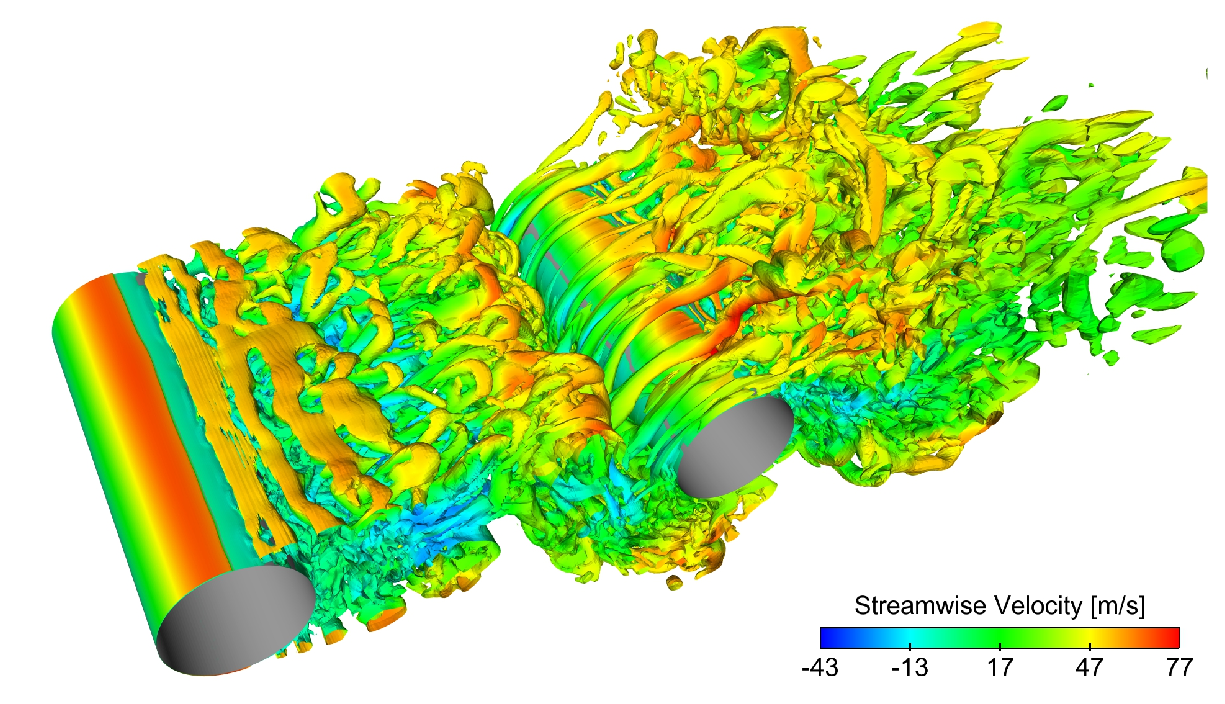
\includegraphics[width=0.40\textwidth]{tc_q_criteria}
    \bicaption{Q判据等值面图,同时测试一下一个很长的标题,比如这真的是一个很长很长很长很长很长很长很长很长的标题。}{Isocontour of Q criteria, at the same time, this is to test a long title, for instance, this is a really very long very long very long very long very long title.}
    \label{fig:tc_q_criteria}
\end{figure}
\section{Improved GOA(IGOA)}

\section{任务调度问题}
\subsection{问题描述}
\subsection{任务调度模型}
\subsection{实验结果}


\section{本章小结}